\documentclass[a4paper,12pt]{report}
\usepackage[utf8]{inputenc}
\usepackage[T1]{fontenc}
\usepackage[ngerman]{babel}
\usepackage[parfill]{parskip}
%\usepackage{eurosans}
\usepackage[top=3cm, left=3cm]{geometry}
\usepackage{setspace}
\usepackage{mdwlist}
\usepackage{graphicx}
\usepackage{eurosym}
\renewcommand*\familydefault{\sfdefault}

\setcounter{secnumdepth}{-1}

\begin{document}

\title{\textbf{Leitfaden für das ESE-Tutorium 2014}\\}
\date{}
\author{von\\Thomas Heinze, Berit Lochner, Denis Stein (2008), \\Marcus Hähnel und Nico Hoffmann (2009), \\Marius Melzer (2010), \\Robert Schädel (2011),\\Sascha Peukert (2013), \\Kilian Költzsch und Marc Satkowski (2014)}
\maketitle

\chapter{Hinweise für Tutoren}
\section{Ansprechpartner}
Kilian (koeltzsch@ifsr.de): 0151/41929976\\
Marc (satkowski@ifsr.de): 0172/8572425 \\
FSR/ESE-Orga (ese-orga@ifsr.de): 0351/463-38226

\section{Über das Tutorium}
\begin{itemize*}
\item Ziel des Tutoriums ist Vermittlung von Informationen rund um das Studium.
\item Der Inhalt dieser Handreichung ist das Minimum, was ihr in den Tutorien vermitteln sollt.
Ihr könnt die Stichpunkte gerne noch mit eigenen Einfällen ergänzen.
\item Die Informationen sollten möglichst \textbf{unparteiisch} und \textbf{nicht wertend} vermittelt werden.
Insbesondere sollte man vermeiden, den Erstis schon vorab Angst vor bestimmten Vorlesungen oder Dozenten zu machen oder sie zum Nichtbesuchen der Vorlesungen zu animieren.
Betrifft vor allem auch das ESE-Spiel.
\item Eine Tutoriengruppe besteht aus zwei Tutoren und ca. 15-25 Erstis.
\item Falls keiner der beiden Tutoren zu einem Thema eine Auskunft geben kann, verweist am besten auf erfahrenere ESE-Tutoren oder den FSR, anstatt (möglicherweise falsche) Spekulationen zu äußern.
Montag Nachmittag wird das FSR-Büro besetzt sein, sodass ihr Leute mit spezifischeren Fragen auf Montag Nachmittag oder die Seminartutorien am Dienstag verweisen könnt.
\item Wie in den letzten Jahren hat jede Gruppe hat einen Namenspatron.
Anhand dessen werden euch die Studenten nach der Begrüßung per Los zugeteilt.
\end{itemize*}

\section{Vor dem Tutorium zu erledigende Dinge}
\begin{itemize*}
\item Lest euch diesen Leitfaden schon mal im Ganzen durch.
Es wäre schlecht, wenn ihr das erst im Tutorium selbst tun müsst!
Markiert euch eventuell wichtige Punkte.
Wenn ihr Fragen habt, stellt diese beim Tutorentreffen oder per Mail.
\item In der unten stehenden Tabelle Ort eures Tutoriums nachsehen.
\item Den Raum bitte vorher schonmal suchen, falls ihr nicht sicher wisst, wo er sich befindet.
\item Am ESE-Montag bitte spätestens um 9:00 da sein und mit helfen (10:00 geht die Begrüßung mit den anschließenden Tutorien los)!
Wir treffen uns in der INF/E023 zum Frühstück.
\item Am Montag um 09:30 ist in der INF/E008 ein letztes Tutorentreffen.
Dort bekommt ihr ein letztes Briefing  und die letzten Gruppen haben die Chance, Helfer zu casten.
\item Überlegt euch zusammen mit eurem Tutoriumspartner, wie ihr die Informationen vortragen wollt.
Möglicherweise wollt ihr bestimmte Dinge an die Tafel schreiben.
Vielleicht ist es am sinnvollsten, die Stichpunkte abwechselnd vorzutragen, damit der jeweils andere sich schon mal Gedanken zum nächsten machen kann.
\item Stellt euch ebenfalls darauf ein, am Dienstag zur \textbf{Übungseinschreibung} zwischen 8:40 und 12:30 Uhr anwesend zu sein und zu helfen.
\end{itemize*}

\begin{center}
\vspace{1cm}
\begin{tabular}[h]{|l|l|l|l|}
	\hline
	\textbf{Namenspatron} & \textbf{Tutor(en)} & \textbf{Raum}\\ \hline
	Edsger W. Dijkstra & Sebastian \& Simon & INF/E005\\
	Kurt Gödel & Marcel \& Markus & INF/E006\\
	Konrad Zuse & Alex \& Ian & INF/E007\\
	Donald Ervin Knuth & 	Katja \& Anna & INF/E008\\
	John von Neumann & Laura \& Tamara & INF/E009\\
	Tim Berners-Lee & Philipp \& Kilian & INF/E010\\
	Alan Turing & Justus \& Felix & SCH/A216\\
	Ada Lovelace & Emma \& Anna & BAR/106\\
	Grace Hopper & Lara \& Ben & JAN/27\\
	Richard Stallman & Axel \& Thomas & BER/105\\
	Linus Torvalds & Manuel \& Richard & SCH/A01\\
	Noam Chomsky & Phillip \& Sven & SCH/A315\\
	Christiane Floyd & Sinthu \& Marius & SCH/A215\\
	Stephen A. Cook & Lisa \& Hung & INF/2101\\
	Ken Thompson & Sarah \& Bettina & SCH/A118\\
	Marc Andreessen & Björn \& Julian & SCH/A316\\
	\hline
\end{tabular}
\end{center}

\chapter{Zu vermittelnde Informationen}

\section{Einführung}
\begin{itemize*}
\item Macht eine kleine Vorstellungsrunde, um euch kennenzulernen und die Atmosphäre ein bisschen aufzulockern.
Die Tutoren beginnen.
Am besten ihr erzählt, wie ihr heißt, wo ihr ursprünglich herkommt, was euch an der (Medien-) Informatik gefällt.
Die Studenten könnten zusätzlich noch erwähnen, was sie vorher gemacht haben und wieso sie sich für das Inf/MInf-Studium in Dresden entschieden haben.
Schreibt am besten an die Tafel, was ihr gerne von den Erstis wissen möchtet.
\item Falls ihr eurer Gruppe anbieten wollt, auch nach dem Tutorium eventuell aufkommende Fragen zu beantworten, schreibt eure Emailadressen an die Tafel.
\item Erzählt etwas zu eurem Namenspatron. Informationen zu diesem findet ihr im Anhang.
\end{itemize*}

\section{ESE-Woche}
\begin{itemize*}
\item ESE-Website: http://ese.ifsr.de (mit aktuellem Ablaufplan der ESE-Woche (da er sich auch in der Woche noch verändern kann), Weblinks, etc.)
\item Den Zeitplan gibt es auch im iCal Format (ICS Datei) auf ese.ifsr.de zum Download.
Kann man sich direkt in den Kalender importieren.
\item Der Ablaufplan der ESE wird am FSR-Büro hinter der Wendeltreppe hängen und auf der ESE-Webseite stehen.
\item Die wichtigen Dinge der ESE-Tüte durchgehen: NoPanic, Stundenplanauswahl, etc.
\item Geht die ESE-Woche durch und sagt kurz etwas zu den wichtigsten Programmpunkten
\item Bitte betont nochmal, dass die ESE sehr gut geeignet ist, um Kommilitonen kennenzulernen.
\end{itemize*}
\vspace{0.5cm}
Ort der Begrüßung ist der Lichtenheldt-Hörsaal im Zeunerbau (Bombentrichter) und der der Vorträge ist die ganze Woche über die INF/E023.

% TODO: Graphischer Zeitplan
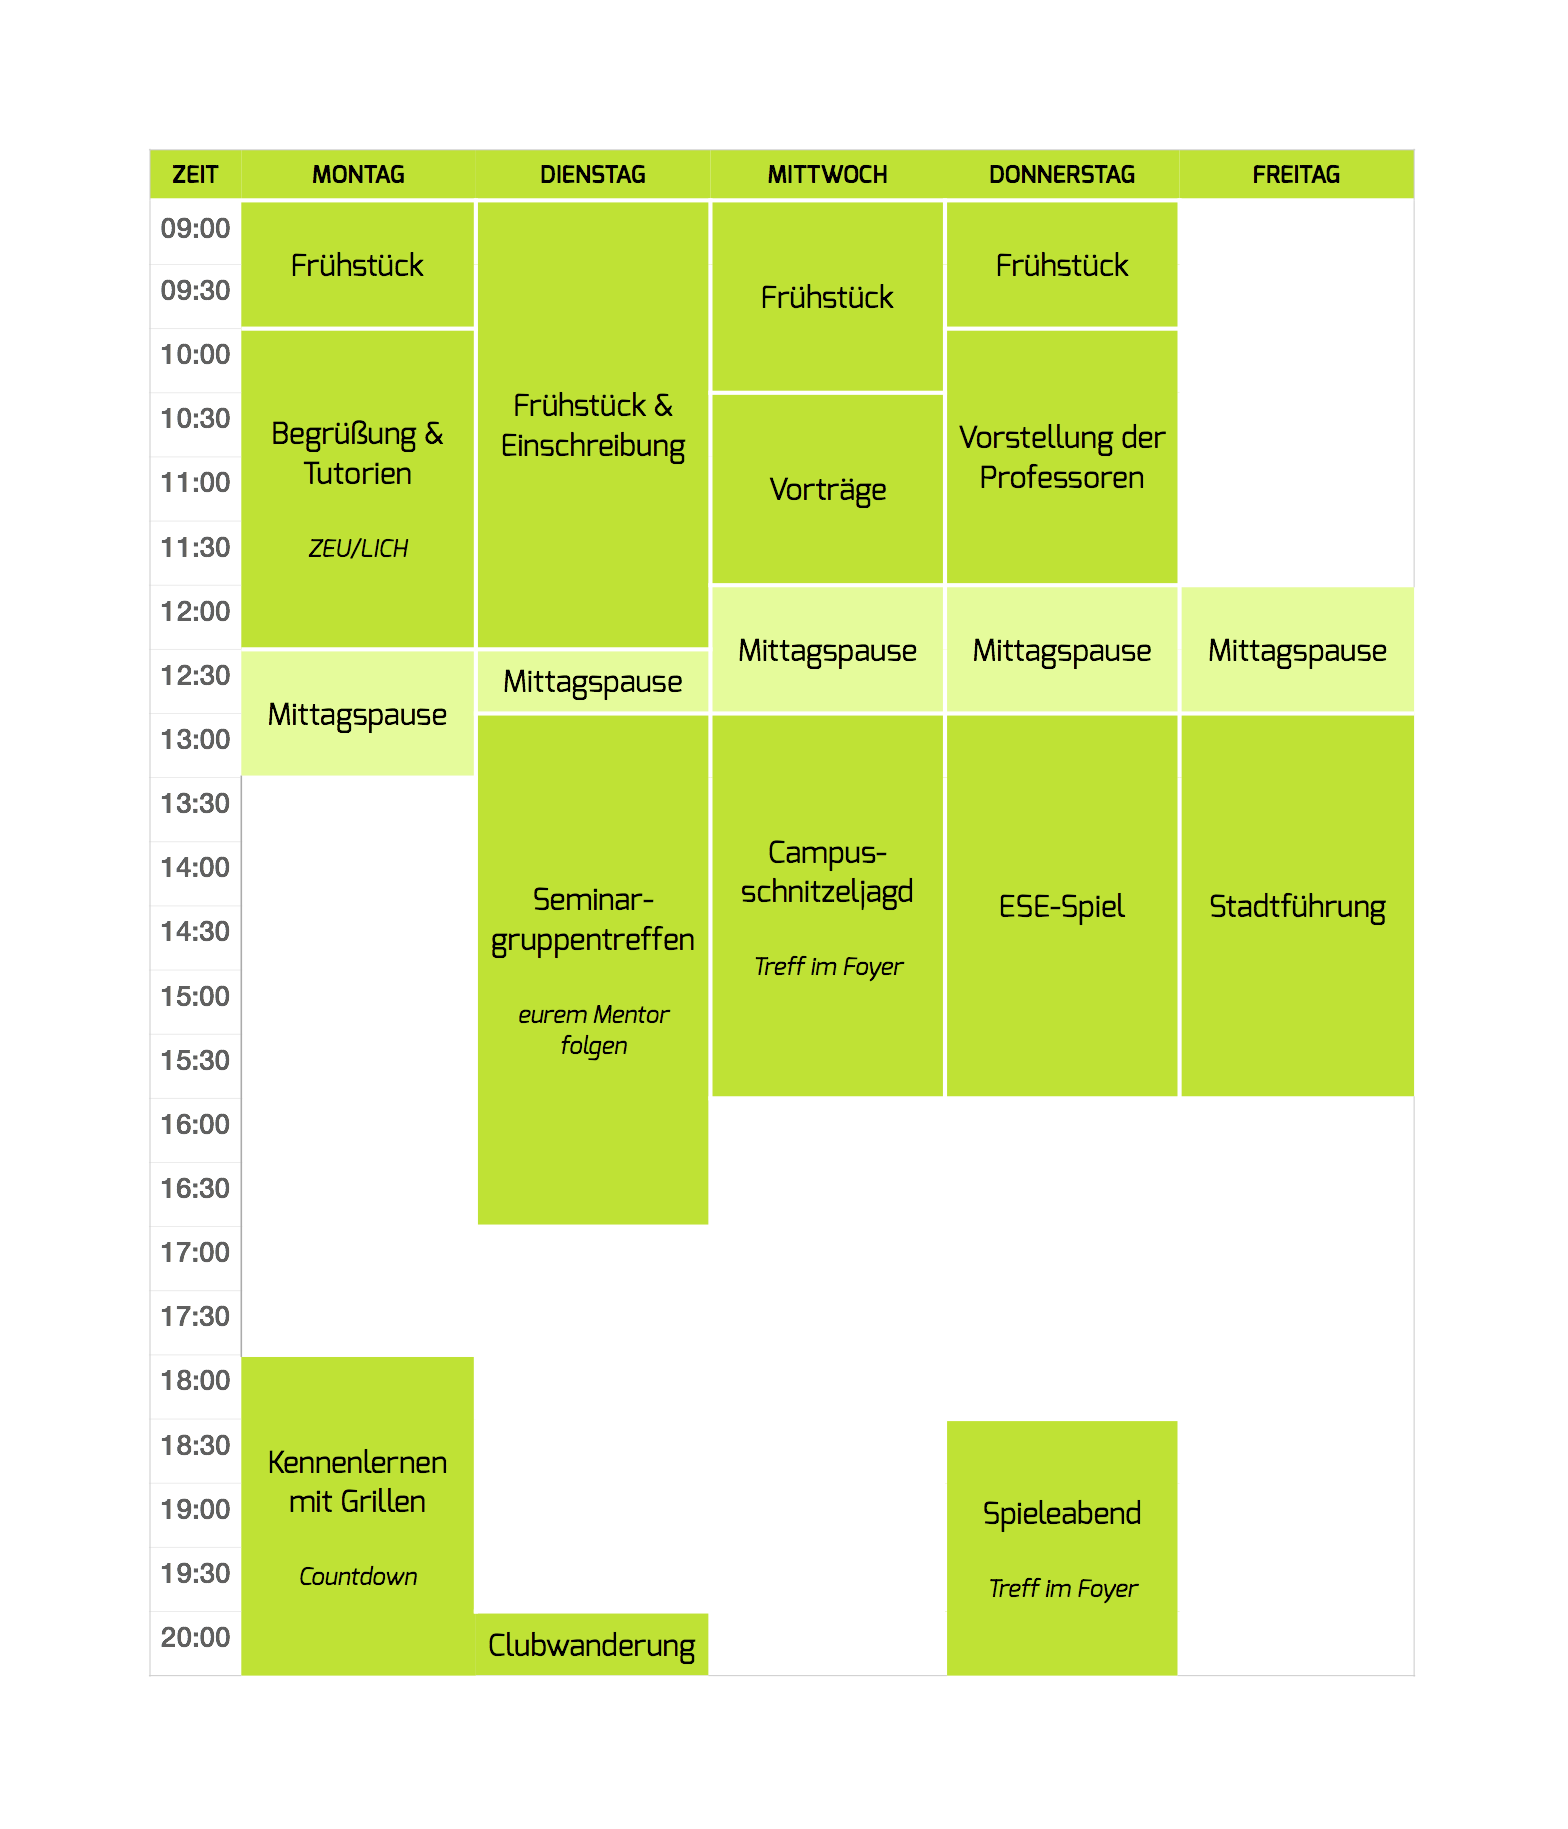
\includegraphics[width=\linewidth]{./zeitplan.png}

\subsection{Montag}
09:00 - 10:00 Frühstück\\
10:00 - 11:00 Begrüßung im ZEU/LICH\\
11:00 - 12:30 Tutorien (siehe Tabelle auf S.2)\\
Seht euch frei darin euren Erstis einen gemeinsamen Mensabesuch im Anschluss an das Tutorium anzubieten.
am Nachmittag Sprechstunde im FSR-Büro\\
Wenn ihr ausländische Studierende in eurer Gruppe habt, erinnert sie bitte an ihre Tutorien am Montag Nachmittag – sie sollten wissen, worum es geht.\\
\\
ab 18:00 Kennlernabend mit Grillen (im Studentenclub Count Down (Güntzstraße 22))\\

\subsection{Dienstag}
09:00 - 12:00 Frühstück und parallel Einschreibung (Wichtig! siehe S.5 )\\
12:30 - 13:00 Mittagspause \\
ab 13:00  Erstes Seminargruppentreffen (Wichtig! siehe S. 5 )
\\
ab 20:00 Clubwanderung (Startet beim Studentenclub Count Down (Güntzstraße 22))\\
Bitte weist darauf hin, dass die Clubwanderung aus Versehen nicht im Zeitplan in der No Panic auftaucht und keinesfalls flach fällt.

\subsection{Mittwoch}
09:00 - 10:30 Frühstück\\
ab 10 Uhr Vortragsfähigkeit der E023 herstellen\\
10:30 - 11:00 Vortrag Studienangelegenheiten und Organisation\\
11:00 - 11:30 Vortrag Auslandsstudium \\
11:30 - 11:45 Vortrag studentische Mitbestimmung \\
11:45 - 12:00 Vortrag TUDIAS \\
12:00 - 13:00 Mittagspause \\
12:40 Helfertreff Schnitzeljagd
13:00 - 16:00 Campus-Schnitzeljagd \\


\subsection{Donnerstag}
09:00 - 10:00 Frühstück\\
10:00 - 12:00 Vorstellung der Professoren\\
12:00 - 13:00 Mittagspause\\
12:40 Helfertreff ESE-Spiel
13:00 - 16:00 ESE-Spiel\\
\\
ab 18:30 Spieleabend in der Fakultät\\

\subsection{Freitag}
13:00 - 16:00 Stadtführung (bitte erfragt grob das Interesse und gebt es weiter an Philipp <heisig@ifsr.de>)\\

\subsection{Einschreibung}
\begin{itemize*}
	\item Treffen am Dienstag am Eingang zum Rechenzentrum.
	\item Jede Gruppe hat einen zugewiesenen Zeitpunkt, an dem sie drankommen. Wichtig: Uhrzeit für euer Gruppe ansagen (Siehe Tabelle auf S. 2)!
	\item Ruhig ein bisschen eher da sein, vor allem gegen Ende geht es meist schneller.
	\item Die Studenten sollten ihren Zettel mit dem Namenspatron unbedingt bis dahin behalten.
	Diesen müssen sie vorzeigen, wenn sie zur Einschreibung erscheinen. Ohne Zettel müssen sie bis zum Ende der Einschreibung warten.
	\item Sollten sich Master in die Tutorien verirrt haben:
	Sie brauchen sich nicht in Seminargruppen einzuschreiben.
	Das gleiche gilt für Lehrämtler und höhersemestrige Quereinsteiger.
	\item Mitzubringen sind:
		\begin{itemize*}
		\item Zettel mit Namenspatron
		\item Studentenausweis
		\item kompletter Semesterbogen (insbesondere wegen Login und Passwort)
		\item Wunschstundenplan (vorher raussuchen, sonst kein Einlass!)
		\item zu beachten ist, dass die Einschreiben nur von der Informatik-Fakultät getan werden kann, sie wird erst am Mittwoch für außerhalb freigeschalten.
	\end{itemize*}
	\item Ihr werdet von den Tutoren gefragt, ob sie euch in die vier folgenden Mailinglisten/Mailverteiler eintragen sollen (bei drei ist es ratsam, bei der auf der Job-Angebote erscheinen sollte jeder selber wissen ob er das braucht):
		\begin{itemize*}
		\item FSR-info ist der Verteiler des FSR über den regelmäßig Informationen zu den Vorgängen an der Fakultät und den Sitzungen des FSR kommen.
		\item inf14-info: Verteiler von Informationen, die konkret den Studiengang der 2014 immatrikulierten Studenten betreffen (erfahrungsgemäß \textit{sehr sehr} wenig Content).
		\item inf14-discuss: Mailingliste zur Diskussion untereinander.
		\item extern: Jobangebote werden über diese Mailingliste verbreitet.
		\item und diverse andere, siehe \\ https://www.ifsr.de/fsr:news:quicklinks\_fuer\_die\_einschreibung
	\end{itemize*}
\end{itemize*}

\subsection{Seminargruppentreffen}
\begin{itemize*}
	\item Allgemeiner Sinn der Seminargruppen: Unterstützung der Erstis, Gruppenbildung, Mentor als Ansprechpartner bei Problemen und Vermittlung aller relevanten Informationen zum Studiengang
	\item \glqq Als Einzelgänger kommt man im Studium nicht weit\grqq
	\item Bitte betonen:
	Seminargruppentreffen vermitteln wichtige Informationen, darum sollte man an allen teilnehmen!
	\item Erstes Seminargruppentreffen ist direkt nach der Einschreibung am Dienstag um 13 Uhr bzw. 15 Uhr (je nach Seminargruppe - genauer Termin wird bei der Einschreibung dann mitgegeben).

\end{itemize*}

\section{Studium}
\subsection{Allgemein}
\begin{itemize*}
	\item Alle wichtigen Informationen bezüglich des Ablaufs des Studiums befinden sich in der Prüfungs- und Studienordnung (Inf-Website -> Studium -> Für Studierende -> Regularien -> Studien- und Prüfungsordnungen).
	In den Anhängen (separate PDFs!) befindet sich jeweils eine nützliche Stundentafel mit den zu Belegenden Fächern geordnet nach Studiensemester.
	Für den Bachelor stehen gute Beschreibungen der einzelnen Module in der Studienordnung - reingucken lohnt sich.
	\item Die studiengangsspezifischen Informationen werden im ersten Seminargruppentreffen näher erklärt
	\item Während des Studiums wird es Vorlesungen, Übungen und Praktika geben, die in Modulen gruppiert sind.

	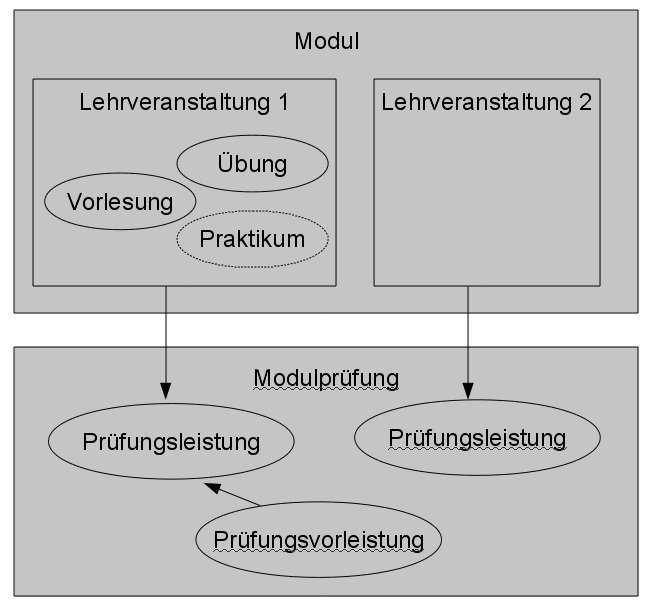
\includegraphics[width=14cm]{modul.jpg}
	\begin{center}
	Die Zeichnung am besten auf die Tafel malen oder was eigenes ausdenken.
	\end{center}

	\item Es gibt allerdings auch viele Module, die nur eine Lehrveranstaltung (Vorlesung + Übung) beinhalten.
	\item Jedes Modul hat eine ausgeschriebene Anzahl an Leistungspunkten (LP).
	Ein Leistungspunkt entspricht einer \glqq Arbeitsbelastung\grqq\ von 30 Stunden über das Semester verteilt.
	Die setzt sich zusammen aus der Präsenzzeit (SWS), der Vor- und Nachbereitung der Lehrveranstaltung, der Vorbereitung auf die Prüfung und der Prüfung selbst.
	Leistungspunkte werden einem erst nach bestandener Modulprüfung angerechnet.
	\item Ein Modul hat eine Modulprüfung (MP).
	Die MP kann aus verschiedenen Prüfungsleistungen bestehen, wobei nicht alle davon zwingend für das Bestehen des Moduls notwendig sind.
	Bei mehreren Prüfungsleistungen wird oft (aber nicht immer, z.B. nicht bei Mathe) das arithmetische Mittel zur Berechnung der Modulnote angewandt.
	Daraus folgt, dass man Module auch mit einer nichtbestandenen Prüfungsleistung bestehen kann, wenn man diese durch eine andere Note ausgleichen kann.
	\item Die Zulassung zu jeder Prüfungsleistung kann theoretisch durch eine oder mehrere Prüfungsvorleistungen (PVL) definiert sein.
	D.h., wenn man die PVL nicht besteht, wird man auch nicht zur Prüfung zugelassen.
	Beispiel: In Mathe muss man Übungen abgeben.
	50\% der Übungspunkte müssen erworben sein, um an der zweiten Prüfung teilzunehmen.
	\item Im Mathe-Modul im ersten Semester gibt es bereits in der Mitte des Semesters eine Prüfungsleistung, zusätzlich zu der am Ende des Semesters.
	Mathe ist im ersten Semester viel Stoff und nicht einfach, das sollte man nicht schleifen lassen!
	\item Eine Vorlesung wird von einem Dozenten, meist einem Professor, gehalten.
	Die meisten Vorlesungen finden im Hörsaalzentrum statt.
	\item Zu fast allen Vorlesungen gibt es zugehörige Übungen, die normalerweise nicht vom Professor, sondern von Mitarbeitern oder Studenten höheren Semesters gehalten werden.
	Fast alle Leute in einer Übungsgruppe sind aus der selben Seminargruppe.
	In den Übungen werden meist ähnliche Aufgaben gelöst, wie sie in den Prüfungen zu erwarten sind.
	Oft wird erwartet, dass man die Übungsaufgaben (meist ein A4-Zettel) vor der tatsächlichen Übung löst.
	In der Übung werden dann die Ergebnisse besprochen.
	\item Praktika sind meist uniinterne, entweder während der Vorlesungszeit oder während der vorlesungsfreien Zeit (dann im zusammenhängenden Block) stattfindende praktische Lernveranstaltungen.
	\item Zum Abschluss einer Lehrveranstaltung findet eine Prüfung des erlernten Stoffes statt.
	Prüfungen liegen im Normalfall in der Kernprüfungszeit, die in den ersten 4-5 Wochen der vorlesungsfreien Zeit liegt.
	Module können mehrere Prüfungen beinhalten.\\
	Prüfungen können zwei mal wiederholt werden.
	Wer durch eine Prüfung fällt, hat ein Jahr (zwei Semester) Zeit, diese zu wiederholen, für die zweite Wiederholung hat man allerdings darauf hin nur ein Semester Zeit.
	Wer die 2. WH (Wiederholungsprüfung) nicht schafft, wird exmatrikuliert und hat somit sein Studium nicht geschafft.
	\item Eine Abmeldung von einer Prüfung ist ohne Angabe von Gründen bis 3 Werktage (bzw. 2 Wochen bei mündlichen Prüfungen) vor dem Prüfungstermin möglich.
	\item Innerhalb der genannten Frist spricht man von Rücktritt.
	Ein Rücktritt ist nur bei Krankheit o.ä. zulässig und muss dem Prüfungsamt unverzüglich schriftlich mitgeteilt werden (ärztliches Attest o.ä.).
	\item Wer eine Prüfung vor dem im Studienablaufplan angegebenen Zeitpunkt absolviert, kann von der Freiversuchsregelung gebrauch machen.
	Siehe \S15 der Prüfungsordnung (Laut Hochschulgesetz abgeschafft, aber da sie noch in der Ordnung steht, gilt die Regelung noch!).
	\item Zu jedem Studiengang gehört ein Prüfungsausschuss.
	An diesen können Anträge auf Anerkennung bzw. Anrechnung von Studien- und Prüfungsleistungen, Anträge auf Prüfungsfristverlängerung, Anträge auf Annullierung einer Prüfung, etc. gestellt werden
	\item Sowohl beim Diplom als auch beim Bachelor darf man die Regelstudienzeit um bis zu 4 Semester überziehen.
	Danach gilt die Abschlussprüfung das erste mal als nicht bestanden.
	\item Man kann seine Studienzeit durch Urlaubs- und Gremiensemester verlängern.
	Ein Urlaubssemester ist ein studienfreies Semester, in dem neuerdings auch Prüfungen geschrieben werden können. 	Gremiensemester sind eine Reduzierung der Fachsemesterzahl.
	Man bekommt sie durch Engagement in den Gremien der Fakultät, z.B. als Mitglied von Fachschaftsrat, Fakultätsrat, Prüfungsausschuss, etc.
	\item Eine Zusammenstellung von fürs Studium wichtigen Dokumenten und Links zu vielen Skripten findet man auch auf der FSR-Seite (ifsr.de -> Studium).
	Diplomer können aufgrund der ähnlichen Lehrveranstaltungen vorerst im Bereich Bachelor nach Skripten gucken, der Bereich \glqq Altes Diplom\grqq\ ist für das \glqq alte\grqq\ Diplom, nicht das neue.

\end{itemize*}

\section{Drucken, Kopieren, Rechentechnik}
\begin{itemize*}
	\item Das Rechenzentrum beinhaltet Computer-Arbeitsplätze, Wlan-Arbeitsplätze (Monitore mit VGA-Eingang, an die man sein Notebook anschließen kann), ein paar Spezialräume mit Multimedia-Equipment und eine Technik-Ausleihe (z.B. für Kameras, Beamer, etc.).
	Die meisten PCs haben einen Dualboot mit Windows und Linux (Ubuntu).
	\item Die Einschreibung in Übungen und Prüfungen und das Abrufen der Prüfungsergebnisse geschieht über das elektronische Einschreibesystem jExam.
	Man findet es unter http://jexam.de.
% TODO: Format der E-Mail Adressen ist jetzt wie?
	\item Jeder Student hat ein Emailpostfach beim ZIH mit der Adresse sNR@mail.zih.tu-dresden.de.
	Neben POP3 und IMAP kann man die Mails auch über das Webinterface unter https://mail.zih.tu-dresden.de abrufen.
	Es ist wichtig, das Postfach regelmäßig abzurufen oder sich die Emails an eine andere Adresse weiterzuleiten, weil unter der Adresse u.a. Informationen über Prüfungsanmeldung, Rückmeldung zum kommenden Semester etc. ankommen.
	\item \textbf{Wichtig!} Falls noch nicht geschehen: Passwort noch heute im IDM ändern, damit morgen die Einschreibung funktioniert: https://idm-service.tu-dresden.de -- ruhig als Hausaufgabe aufgeben.
	\item Es gibt zwei WLAN-Netze auf dem Universitätsgelände.
	Das einfacher einzurichtende, aber unsicherere VPN/Web und das auch an anderen Universitäten (auch international) verwendete Eduroam.
	VPN/Web ist ein offenes Netzwerk.
	Nach dem Verbinden muss man seine Login-Daten nach dem Aufrufen der ersten Website im Browser eingeben.
	Zum Verwenden von Eduroam sollte man die Anleitung auf der Website der TU Dresden lesen und sich falls notwendig das benötigte Zertifikat herunterladen.
	Unter Linux funktioniert es mittlerweile mit allen wichtigen Networkmanagern (Gnome Network Manager, KNetworkmanager, wicd, auf der Konsole per wpasupplicant..).
	Unter aktuellen Versionen von Windows und OS X reicht es sich mit dem ZIH Login anzumelden.
	\item Der ZIH-Login gilt sowohl fürs Rechenzentrum als auch für jExam, Email und WLAN.
	Username ist die \glqq sNr\grqq, die auf den Immatrikulationsbögen steht.
	Passwort für den Erstlogin steht dort ebenfalls, ist aber wie bereits erwähnt dringendst abzuändern, da jegliche Funktionalität sonst stark eingeschränkt ist.
	\item Drucken und Kopieren ist möglich im FSR-Büro (ab 2ct/Seite), über eine beim Stura zu erwerbende Kopierkarte an unterschiedlichen Standorten in der Uni (http://www.fritzsche-steinbach.de/Download/Flyer\_TU\_Dresden.pdf -- 3,7-5ct/Seite), in der SLUB (5-15ct/Seite) oder an den diversen Copyshops auf dem Unigelände.
\end{itemize*}

\section{Studentische Selbstverwaltung}
\subsection{Fachschaftsrat}
Der Fachschaftsrat ist die Vertretung der Studenten auf Fakultätsebene.
Er besteht derzeit aus 17 Mitgliedern und wird immer im Wintersemester für ein Jahr neu gewählt.
Der FSR ist Ansprechpartner bei Fragen und Problemen und veranstaltet die ESE, Professorenstammtische, die Spieleabende, die Lehrevaluationen und diverse Turniere.
Die FSR-Sitzungen sind jede Woche Montags um 18:30 im Großen Ratssaal INF/1004 in der ersten Etage.
Die Sitzungen sind öffentlich, Gäste sind herzlich willkommen und die Protokolle findet man auf dem FTP-Server (ftp://ftp.ifsr.de), genauso wie Klausuren vergangener Jahre oder (fürs Hauptstudium / Master) Komplexprüfungsprotokolle.
Der FSR hat sein Büro in der INF/E017 (hinter der Treppe, neben dem Cafe ASCII).
Auf der Website ifsr.de gibt es Informationen zum Studium und Neuigkeiten rund um die Fakultät.
Auch als Ersti kann man sich gerne für den nächsten FSR zur Wahl stellen. Als Tutor natürlich erst recht :)

\subsection{Studentenrat}
Der Studentenrat, kurz StuRa, ist die Vertretung der Studenten auf Uniebene.
Er versucht studentische Interessen gegenüber der Universitätsleitung durchzusetzen, er verteilt Gelder und bietet Beratung zu BAföG, Sozialem und bei Rechtsfragen/-problemen.
Die Mitglieder sind Entsandte aus den FSRen der einzelnen Fakultäten.
Auch die Sitzungen des StuRa sind öffentlich und finden zweiwöchentlich an Donnerstagen ab 19:30 Uhr statt.

\section{Studentisches Leben}
\subsection{Studentenclubs}
In Dresden gibt es 16 Studentenclubs, die von ehrenamtlich von Studenten geführt werden.
Eine Auflistung gibt es z.B. unter http://www.vdsc.de (Vereinigung Dresdner Studentenclubs).
Der Studentenclub, der zur Fakultät Informatik \textit{gehört}, ist das \glqq CountDown\grqq\ in der Nähe des Straßburger Platzes.
\subsection{Kino}
Das Kino im Kasten ist ein Studentenkino und befindet sich an der Philosphischen Fakultät in der August-Bebel-Straße.
Mehr Informationen und das Kinoprogramm gibts unter http://kino-im-kasten.de.
Das KiK hat seit kurzem wieder geöffnet und freut sich über Besucher.

\section{Die Universität}
\subsection{SLUB}
Bei der Sächsischen Landes- und Universitätsbibliothek kann man sich als Student kostenlos anmelden und Bücher ausleihen oder sich in die ruhigen Räumlichkeiten zum Lernen setzen.
Die meisten Informatikbücher befinden sich in der Lehrbuchsammlung im Haupthaus und im gegenüberliegenden \glqq DrePunct\grqq.
\subsection{Mensen}
In allen Mensen der TU Dresden (Alte Mensa, Reichenbachstraße, Siedepunkt, Zeltmensa ...) kann man mit der \glqq Emeal\grqq-Karte bezahlen, die sich per Barzahlung an den Kassen, im Voraus per Kontozahlung am Automaten aufladen lassen oder per Selbstaufladung vom Konto bei Bedarf.
Die Mensakarten werden während der ESE beim Frühstück für einen Pfand von 5 Euro ausgegeben;
Wer noch keinen hat, kann auch im FSR-Büro vorbeikommen.

\subsection{Unisport}
Im Universitätssportzentrum kann man aus einer großen Anzahl von Sportarten wählen.
Die Einschreibung findet auf der Website des USZ (http://tu-dresden.de/ die\_tu\_dresden/zentrale\_einrichtungen/usz/) am Dienstag, den 14.10.2014 je nach Sportart ab 17.00 oder später statt.

\subsection{Sprachkurse}
Insgesamt bis zu 10 SWS Sprachkurse kann man kostenlos beim Sprachenzentrum LSK belegen.
Man kann je nach Kurs Sprachzertifikate bekommen oder einfach mal eine neue, fremde Sprachen erlernen.
Für den Informatik-Master wird Englisch benötigt.
Website: http://lskonline.tu-dresden.de.

\subsection{Nebenjobs}
SHKs (Studentische Hilfskräfte) werden überall an der Uni gesucht.
Viele informatikbezogene werden in der Fakultät per Aushang beworben oder über Ausschreibungen auf der Informatik Fakultätsseite.

\section{Wohnen in Dresden}
\begin{itemize*}
	\item Wenn man in Dresden seinen Hauptwohnsitz anmeldet bekommt man ein \glqq Begrüßunggeld\grqq\ von 150 Euro, das man beim Studentenwerk beantragen kann.
	\item Zweitwohnungssteuer: in Dresden fällig seit 2006, 10\% der jährlichen Netto-Kaltmiete (aber nur wenn echte Zweitwohnung; http://www.dresden.de/media/ pdf/infoblaetter/Handzettel\_Info\_Zweitwohnungssteuer.pdf).
	Als Bewohner einer WG oder eines Wohnheimes kann man allerdings Widerspruch einlegen und muss die Steuer nicht zahlen.
	\item Den neuen Wohnsitz sollte man innerhalb von 14 Tagen bei den Meldestellen angeben (http://dresden.de/de/02/or/anliegen/c\_241.php).
	\item Im Studentenheim sind am Anfang des Semesters meist bereits keine Plätze mehr frei.
	Fragen kann man aber trotzdem.
\end{itemize*}

\section{Dresden}

\subsection{Altstadt}
\begin{itemize*}
	\item Kulturelles Zentrum: Semperoper, Zwinger, Frauenkirche,...
	\item Einkaufsmeile
\end{itemize*}

\subsection{Neustadt}
\begin{itemize*}
	\item Kneipenviertel
	\item viele Programmkinos: Schauburg, Casablanca, Thalia,...
	\item einmal im Jahr großes Straßenfest: BRN - Bunte Republik Neustadt.
\end{itemize*}

\section{Ansprechpartner bei Problemen}
\begin{itemize*}
	\item FSR: fsr@ifsr.de
	\item Studiendekan: Prof. Weber (allgemein), Prof. Friedrich (Lehramtsstudiengänge), Prof. Hölldobler (englischsprachige Studiengänge).
	\item Studentische Studienberatung: Sascha Peukert (studienberatung-inf@ifsr.de) und Kilian Költzsch (studienberatung-minf@ifsr.de) oder beide unter studienberatung@ifsr.de.
	\item studentische Vertreter im Prüfungsausschuss: Sascha Peukert, Duc Tien Nguyen.
	\item Prüfungsamt (INF/3039 und 3040).
	\item Rechtsverbindliche Auskünfte gibt es aber nur vom Prüfungsausschuss, Anträge über das Prüfungsamt stellen!
\end{itemize*}

\section{Rundgang durch die Fakultät}
Macht einen kleinen Rundgang durch die Fakultät und zeigt mindestens: ASCII, FSR-Büro, E023 (Vorlesungssaal), Rechenzentrum, Prüfungsamt.
Anschließend könnte man in die Alte Mensa mensen gehen.

\chapter{Namenspatrone}
\section{Alan Turing (1912 - 1954)}
\begin{itemize*}
	\item Engländer
	\item schuf Großteil der theoretischen Grundlagen der modernen Informatik
	\item unterstützte Entschlüsselung der Enigma
	\item schrieb das erste Schach-Computerprogramm
	\item entwickelte ein Testverfahren, welches herausfinden kann, ob eine Maschine intelligent ist (Turing-Test)
	\item ``Oscar'' der Informatik nach ihm benannt (Turing-Preis)
	\item Studium: Turing-Maschine (GThI)
\end{itemize*}

\section{Edsger W. Dijkstra (1930 - 2002)}
\begin{itemize*}
	\item Niederländer
	\item Djikstra-Algorithmus zur Berechnung des kürzesten Wegs in einem Graphen
	\item Semaphore zur Synchronisation von Threads
	\item berühmt wegen Abhandlung ``Goto considered harmful''
	\item Einführung der strukturierten Programmierung (verwendet in Programmiersprachen wie Pascal oder C)
	\item Studium: Dijkstra-Algo (A\&D), Semaphore (BS)
\end{itemize*}

\section{Kurt Godel (1906 - 1978)}
\begin{itemize*}
	\item Deutscher
	\item Beiträge zur Relativitätstheorie und klassischen Logik
	\item viele Beiträge zur Prädikatenlogik (Vollständigkeit und Entscheidungsproblemen)
\end{itemize*}

\section{Konrad Zuse (1910 - 1995)}
\begin{itemize*}
	\item Deutscher
	\item gilt als Erfinder des modernen Computers
	\item Konstruktion der Computer Z1 bis Z4
	\item Entwicklung der ersten höheren Programmiersprache Plankalkül
	\item theoretische und praktische Arbeit zur Darstellung von Gleitkommazahlen (Exponent, Mantisse)
	\item Studium: Gleitkommazahlen (RA1, RAO), Vektorrechner (RA2)
\end{itemize*}

\section{Donald Ervin Knuth (geb. 1938)}
\begin{itemize*}
	\item Amerikaner
	\item Verfasser von ``The art of Computer programming'' (Standardwerk über Datenstrukturen \& Algorithmen)
	\item entwickelte Satzsystem TeX
	\item Erfinder des KMP-Algorithmus (String Matching) und des Buddy-Verfahrens (Speicherverwaltung)
	\item Studium: KMP (A\&D), Buddy (BS)
\end{itemize*}

\section{John von Neumann (1903 - 1957)}
\begin{itemize*}
	\item Österreich-Ungar
	\item Beiträge in Quantenmechanik und Spieltheorie
	\item Entwicklung der von-Neumann-Architektur
	\item entdeckte während seiner Arbeit an der von-Neumann-Architektur viele Programmkonstrukte: linked subroutines, lists, Einführung der binären Kodierung, double precision arithmetic, Mergesort etc.
	\item Studium: von-Neumann-Architektur (GTeI), Binäre Kodierung, Double precision arithmetic (beides RA1)
\end{itemize*}

\section{Tim Berners-Lee (geb. 1955)}
\begin{itemize*}
	\item Engländer
	\item gilt als Begründer des WWW (Web-Developer, höhö)
	\item erfand HTML
	\item schrieb den ersten Browser
	\item Vorsitzender des W3C (Gremium, welches grundlegende Standards des Netzes spezifiziert)
	\item Studium: WWW (RN)
\end{itemize*}

\section{Ada Lovelace (1815 - 1852)}
\begin{itemize*}
	\item Engländerin
	\item gilt als erste Programmiererin der Welt
	\item beschrieb, wie man die Bernoulli-Zahlen mit einer Maschine berechnen kann
	\item Namensgeberin der Programmiersprache Ada
\end{itemize*}

\section{Grace Hopper (1906 - 1992)}
\begin{itemize*}
	\item Amerikanerin
	\item 1954 ersten Compiler (A-0) entwickelt
	\item Mitarbeit am Mark I und Mark II
	\item fand den ersten (Hardware) Bug (heißt Bug, weil es eine Motte war)
	\item Studium: Entwicklung der Rechentechnick
\end{itemize*}

\section{Richard Stallman (geb. 1953)}
\begin{itemize*}
	\item Amerikaner
	\item Präsident der Free Software Foundation
	\item entwickelte die GPL
	\item entwickelte die ersten Versionen des gcc, gdb und von GNU Emacs
\end{itemize*}

\section{Linus Torvalds (geb. 1969)}
\begin{itemize*}
	\item Finne
	\item Initiator des freien Kernels Linux
	\item bis heute einer der führenden Entwickler von Linux
	\item Studium: Linux (BS)
\end{itemize*}

\section{Noam Chomsky (geb. 1928)}
\begin{itemize*}
	\item Amerikaner
	\item Beiträge in versch. Bereichen wie Linguistik und Psychologie
	\item Chomsky-Hierarchie teilt formale Sprachen in Klassen (Typ 0 bis Typ 3) ein
	\item wichtige Grundlage der Theoretischen Informatik, speziell des Compilerbaus
	\item Studium: Chomsky-Hierarchie (GThI)
\end{itemize*}

\section{Christiane Floyd (geb. 1943)}
\begin{itemize*}
	\item Österreicherin
	\item erschuf die erste Entwicklungsumgebung Maestro I
	\item erste Professorin im Bereich Informatik in Deutschland
	\item umfangreiche Forschung im Bereich von Softwarentwicklungsmethoden
\end{itemize*}

\section{Stephen A. Cook (geb. 1939)}
\begin{itemize*}
	\item Amerikaner
	\item forscht hauptsächlich im Bereich der Theoretischen Informatik
	\item formulierte in seinem berühmtesten Paper den Begriff NP-Vollständigkeit
	\item in diesem Paper lässt er die Frage offen, ob P=NP, welches eine der zentralen Fragestellung der modernen Informatik ist
	\item Studium: P=NP, NP-Vollständigkeit (beides GThI)
\end{itemize*}

\section{Ken Thompson (geb. 1943)}
\begin{itemize*}
	\item Amerikaner
	\item entwickelte Programmiersprache B (Vorgänger von C)
	\item erschuf mit Ritchie erste Version von UNIX
	\item ebenfalls Arbeit an BS Multics und Plan9
	\item schrieb frühe Versionen von Tools wie der ersten Shell sh, die bis heute Bestandteil moderner Betriebssysteme sind
	\item Studium: Unix (BS)
\end{itemize*}

\section{Marc Andreessen (geb. 1971)}
\begin{itemize*}
	\item Amerikaner
	\item Mitbegründer der Netscape Corp.
	\item schrieb einen der ersten weit verbreiteten Browser Mosaic
	\item entwickelte mit am Netcape Navigator, der die Grundlage vom Mozilla Firefox ist
\end{itemize*}

\section{Rudolf Bayer (geb. 1939)}
\begin{itemize*}
	\item Deutscher
	\item forscht im Bereich der Datenbanken
	\item entwickelte Datenstruktur B-Bäume (Grundlage der meisten modernen Datenbank- und Dateisysteme)
	\item Studium: B-Bäume (DB)
\end{itemize*}

\section{Dennis Ritchie (1941 - 2011)}
\begin{itemize*}
	\item Amerikaner
	\item entwickelte mit Thompson Unix
	\item erschuf Programmiersprache C
	\item Studium: C (A\&D), Unix (BS)
\end{itemize*}

\section{Claude Shannon (1916 - 2001)}
\begin{itemize*}
	\item Amerikaner
	\item beschäftigte sich mit mathematischen Grundlagen der Kommunikation
	\item Einführung von verschiedenen Begriffen/Theoremen wie Entropie und Nyquist-Shannon-Abtasttheorem
	\item Studium: Nyquist-Shannon-Abtasttheorem (RN, IKT, EMI, MUMS), Entropie, Shannon-Fano-Verfahren (beides IKT, EMI, MUMS)
\end{itemize*}

\section{C.A.R. Hoare (geb. 1934)}
\begin{itemize*}
	\item Brite
	\item beschäftigte sich mit den theoretischen Grundlagen von Programmiersprachen
	\item entwickelte Hoare-Kalkül (Korrektheit von Algorithmen)
	\item erfand Quicksort
	\item Studium: Hoare-Kalkül (Programmierung), Quicksort (A\&D)
\end{itemize*}

\section{Alonzo Church (1903 - 1995)}
\begin{itemize*}
	\item Amerikaner
	\item Mathematiker und Logiker
	\item hat 1930 u.a. das Lambda-Kalkül erfunden, welches die Grundlage für funktionale Programmiersprachen darstellt
	\item Studium: Lambda-Kalkül (Programmierung)
\end{itemize*}

\end{document}
